% !TeX root = ./10-handout.tex

%\item<2-> % reveals second and keeps on page in subsequent frames
%\begin{itemize}[<2->] %does for a whole list of items

%could do reductio proofs! 
%changes to notion of rigor in mathematics; e.g. bolzano moving away from physical intuition , motion, passage of time. 

%would be neat to discuss curry-howard isomorphism in the context of intuitionistic logic! 


\setcounter{section}{9} 

\section{Incompleteness}
%\subsection*{test}

\begin{frame}
%\large

\scriptsize{\tableofcontents}

\end{frame}

%\iffalse %start of day one stuff 


\begin{frame}
\frametitle{Liable to forget:}
%\large

\begin{itemize}[<+->]

\item Hunt's office hours today are after class and 2:30--3:25pm

\item PSet 9 is due this Sunday (no Canvas quiz component)

\item Evals go live tm morning! (May 5th)

\item[] -- Upload screenshots of BOTH completion pages to earn: % the following:

\item[] -- 1 freebie recitation absence (so $\sim$a gradepoint)

\item[] -- either a lecture attendance or 7.5 points back on a pset

%\item[] -- (so if you attempt 15pts worth of a question on PSet 9 or 10, you'd get full points)


\end{itemize}
\end{frame}

\subsection{Logic \& Languages}

\begin{frame}
\frametitle{Arithmetical Languages}
%\large

\begin{itemize}[<+->]

\item Our goal is to define a language $L$ rich enough to express elementary arithmetic (i.e. natural numbers with addition and multiplication)

\item This will be a ``first-order language'' with identity predicate, equipped with some non-logical symbols for arithmetical functions 

\item NB: if our language were weaker in various ways, then axiomatizations of it would evade incompleteness 
% we'll discuss this on philosophy day!

\end{itemize}
\end{frame}

\begin{frame}
\frametitle{First-order Languages (FOLs) in general}
%\large

\begin{itemize}[<+->]

\item \emph{First-order language \metav{L}}: a set of well-formed formulae (wffs) specified by a recursion clause (building up larger wffs from basic ones), where the symbols include:

% like the one we gave for QL, where the symbols of \metav{L} include: 

\bi 

%\item variables $w, x, y, z$ (possibly with subscripts $n \in \mathbb{N}$) 

\item Variables: $w, x, y, z$ (allowing subscripts $n \in \mathbb{N}$) 
\item Operators: five sentential connectives and two quantifiers
\item Punctuation: left and right parentheses
\item \textcolor{OGlyallpink}{Names}: a set of constants (allowing subscripts $n \in\mathbb{N}$)
\item \textcolor{OGlyallpink}{Predicates}: a non-empty set of capital letters (allowing subscripts), each with ``an invisible label" giving its arity \\ (e.g. 0-place, 1-place, 2-place, etc.) 
\item a set of \textcolor{OGlyallpink}{function} symbols $f(c)$ (syntax: $f$ maps terms to terms) 
% notice that we won't get into trouble syntactically, since we otherwise have never placed parentheses after a lowercase roman letter! So we can add this syntactic stipulation to our recursion clause
\ei 

\item \textcolor{OGlyallpink}{Different} FOLs differ in their names, predicates, and functions

\end{itemize}
\end{frame}

\begin{frame}
\frametitle{First-Order Logic (FOL) with Identity}
%\large


%the only logical predicate in the language is identity 

\[
\begin{array}{cc}\label{gloss:logica-symb}
 \text{{Logical Symbol}}  &\text{{Read}}   \\
\hline
  \text{\footnotesize $=$}  & \text{\footnotesize  \dots is identical to \dots}  \\ \pause
 \text{\footnotesize $\neg$} & \text{\footnotesize  it is not the case that \dots}  \\ \pause
\text{\footnotesize $\&$}  & \text{\footnotesize  it is both the case that \dots and \dots}  \\ \pause
\text{\footnotesize $\forall$} & \text{\footnotesize  every number is such that \dots} \\ \pause
\text{\footnotesize $x_n$ (for $n \in \mathbb{N}$)} & \text{\footnotesize `it'/something} 
\end{array}
\]
\pause
\[
\begin{array}{cc}
 \text{{Auxiliary Symbol}} & \text{{Meaning}}  \\
\hline
 \text{\footnotesize $($} &\text{\footnotesize [left parenthesis]}\\   
  \text{\footnotesize $)$} &\text{\footnotesize [right parenthesis]}
\end{array}
\]
\pause
\begin{itemize}[<+->]

\item The quantifer `$\forall$' takes us from propositional/sentential logic to first-order/predicate logic 
\end{itemize}


\end{frame}

\begin{frame}
\frametitle{Adding in Arithmetic to form $L$}
%\large

\begin{itemize}[<+->]

\item $L$ contains the preceding logical symbols and the following arithmetical symbols:
\end{itemize}
%\pause
\[
\begin{array}{cc}\label{gloss:exponentiation}
 \text{{Arithmetical Symbol}} &\text{{Denotes}}   \\
\hline
 \text{\footnotesize 0}   & \text{\footnotesize  the number zero}  \\ \pause 
  \text{\footnotesize 1}  & \text{\footnotesize  the number one}  \\ \pause 
    \text{\footnotesize $+$}  & \text{\footnotesize  addition}  \\ \pause 
        \text{\footnotesize $\times$}  & \text{\footnotesize  multiplication}  \\ \pause 
            \text{\footnotesize $\wedge$}  & \text{\footnotesize  exponentiation} 
\end{array}
\]



\end{frame}

\begin{frame}
\frametitle{Logical Abbreviations}
%\large

\begin{itemize}[<+->]

\item An \emph{abbreviation} is a notational \textit{shortcut} to make it easier for us to keep track of certain strings of symbols on our official list. 
\end{itemize}
 \pause 
\[
\begin{array}{c|c|c}
 \text{{Abbreviation}}  &\text{{Read}} &\text{{Official Notation}}   \\
\hline
\text{\footnotesize $A \vee B$}  & \text{\footnotesize  $A$ or $B$}  & \text{\footnotesize  $\neg(\neg A  \ \& \ \neg B)$} \\ \pause 
\text{\footnotesize $A \supset B$}  & \text{\footnotesize  if $A$, then $B$}  & \text{\footnotesize  $\neg A  \vee B$} \\ \pause 
\text{\footnotesize $\exists x_i$}  & \text{\footnotesize  some number is such that it}  & \text{\footnotesize  $\neg \forall x_i \neg$} \\ 
\end{array}
\]


\end{frame}

\begin{frame}
\frametitle{Arithmetical Abbreviations}
%\large

%\begin{itemize}[<+->]
%\end{itemize}

\[
\begin{array}{c|c|c}
\text{{Abbreviation}}  & \text{{Read}} & \text{{Official Notation}}     \\
\hline
\text{\footnotesize  $2$} & \text{\footnotesize two} & \text{\footnotesize $(1+1)$}   \\ \pause 
\text{\footnotesize  $3$} & \text{\footnotesize three} & \text{\footnotesize $((1+1) +1)$}  \\ \pause 
\text{\footnotesize $4$} & \text{\footnotesize four} & \text{\footnotesize $(((1+1) +1) + 1)$}   \\  \pause 
\text{\footnotesize \vdots} & \text{\footnotesize \vdots} & \text{\footnotesize \vdots} \\
\end{array}
\]
 \pause 
\[
\begin{array}{c|c|c}
 \text{{Abbreviation}}  &\text{{Read}} &\text{{Official Notation}}   \\
\hline
\text{\footnotesize $x_i < x_j$}  & \text{\footnotesize  $x_i$ is smaller than $x_j$}  & \text{\footnotesize  \(\exists x_k( (x_j = x_i + x_k) \ \& \ \neg(x_k = 0))\)}\\ \pause 
\text{\footnotesize $x_i |  x_j$}  & \text{\footnotesize  $x_i$ divides $x_j$}  & \text{\footnotesize  \(\exists x_k (x_k \times x_i = x_j)\)}\\ \pause 
\text{\footnotesize $\text{Prime}(x_i)$}  & \text{\footnotesize  $x_i$ is prime}  & \text{\scriptsize  \((1< x_i) \ \&\ \forall x_j\forall x_k((x_i = x_j\times x_k)\supset(x_i=x_j\vee x_i=x_k))\)}\\
\end{array}
\]

\end{frame}

\subsection{Are we Rich enough yet?}

\begin{frame}
\frametitle{What does it take to be `rich enough'?}
%\large

\begin{itemize}[<+->]

\item $\mathcal{L}$ counts as ``rich enough'' if one can prove:

\item That language $\mathcal{L}$ is happy and loved! Duh! %(No \$ no problems)

\item \emph{Lemma}: $\mathcal{L}$ contains a formula (abbreviated ``\(\mbox{Halt}(k)\)"), which is true if and only if the $k$th Turing Machine halts on input \(k\).

\item[] -- i.e. $\mathcal{L}$ can \emph{express} \(\mbox{Halt}(k)\) (an uncomputable function)

\item \emph{To express}: a language \emph{expresses} a function $f(n)$ just in case it includes a formula $\phi(x, y)$ s.t. $\phi(n, m)$ is true iff $f(n) = m$

\item[] -- e.g. $\phi(x_1, x_2) := (x_1 +1 = x_2) $ \textit{expresses} the successor function $S(k) = k+1$

\end{itemize}
\end{frame}

\begin{frame}
\frametitle{Halting Function recap}
%\large

\begin{itemize}[<+->]

\item Recall the Halting Function: 

\item $
H'(n,m) =
\begin{cases}
1 \text{\quad if the \(n\)th Turning Machine halts when given input \(m\);}\\
0 \text{\quad otherwise.}
\end{cases}$
%\vspace{1mm}

\item For instance: $H'(2310, 0)=0$ and $H'(2310, 2310)=1$.

\item[] -- where `2310' codes the Turing machine 0 \, \ub \, \ub \, r \, 0
%which doesn't halt if fed empty string; just goes right forever
%but halts if fed a non-empty string, since state 0 is not told what to do w/ a 1 on the tape 

\item Since the `diagonal' entries matter most, we let $\emph{H(n)}:= H'(n,n)$

\item[] -- e.g. $H(2310)=1$


\end{itemize}
\end{frame}

\begin{frame}
\frametitle{The Halting Function is not Turing-Computable}
%\large

\begin{itemize}[<+->]

\item Assume for \emph{reductio} that $\exists$ an \(M^{H}\) that computes \(H(n)\). 

\item Construct Turing Machine \(M^I\) that behaves as follows on input $k$:

\begin{description}
\item[Step 1:] Check whether $H(k)$ (using \(M^H\)). 

\item[Step 2:] 
$\begin{cases}
\text{If $H(k)=1$, go right forever.} \\

\text{If  $H(k)=0$, halt}.

\end{cases}$
\end{description}

\item Consider what happens when we run \(M^I\) on its Turing number $\overline{M^I}$:
%note that this is exactly what $H(\overline{M^I}) = H' (\overline{M^I}, \overline{M^I}) computes, i.e. runs the input \overline{M^I} on the M^I-th turing machine 

\item If $H(\overline{M^I}) = 1$. Then (by Step 2) $M^I$ goes right forever on input $\overline{M^I}$. So $H(\overline{M^I}) = H'(\overline{M^I}, \overline{M^I})= 0$. Contradiction!

\item If $H(\overline{M^I}) = 0$. Then (by Step 2) $M^I$ halts on input $\overline{M^I}$. So $H(\overline{M^I}) = 1$. Contradiction!


\end{itemize}
\end{frame}

\begin{frame}
\frametitle{Incompleteness$_1$: quick proof sketch}
%\large

\begin{itemize}[<+->]

\item NB: for question 6 on PSet 10, see the relevant page on MITx for more precise proof to modify! 

\item Assume that the lemma holds: $\mathcal{L}$ contains a formula \(\mbox{Halt}(k)\), which is true if and only if the $k$th Turing Machine halts on input \(k\)

\item Goal: show that no TM, when given an arbitrary sentence $\phi$ of $\mathcal{L}$, outputs a `1' if $\phi$ is true and a `0' if $\phi$ is false. 

\item Assume for contradiction that such a Machine $M$ DOES exist. 

\item Then we could feed into $M$ the sentence \(\mbox{Halt}(k)\), for any $k$. \\ $M$ would then tell us whether this sentence is true (or false)
\item[] which by the lemma is equivalent to telling us whether the $k$-th Turing Machine halts on input $k$

\item[] -- So $M$ would compute the Halting function, which we know is impossible

\item Conclusion: no such $M$ can exist (proving Incompleteness$_1$)

\end{itemize}
\end{frame}

% %if time/energy: sketch more involved/detailed proof of version 2, which students might like better. Since it involves running a TM for arbitrarily long, having it output all and only the true sentences of language \mathcal{L}. and this seems like something we could set up

%question: what is connection b/w first-order logic being complete but undecidable vs. arithmetic being incomplete (and seemingly also undecidable)?

\begin{frame}
\frametitle{Doing the Work}
%\large

\begin{itemize}[<+->]

\item Lemma: $\mathcal{L}$ contains a formula \(\mbox{Halt}(k)\), which is true if and only if the $k$th Turing Machine halts on input \(k\)

\item So the real work is in showing that the lemma holds for some interesting languages



\item We will sketch how to show the lemma holds for the language $L$ of elementary arithmetic

\item[] --Need to show how to express \textrm{Halt(k)}
 in arithmetic $L$

\item The lemma does not hold for some weaker languages that give rise to complete theories of fragments of arithmetic
%/theories, which are in fact complete

\end{itemize}
\end{frame}

\begin{frame}
\frametitle{Philosophy Prompt \#22: Reformulations?}
%\large

\begin{itemize}[<+->]

\item At the core of Incompleteness proofs is the use of arithmetic to express a variety of claims that do not seem to intrinsically be \textit{about} arithmetic. 

\item We use numbers to `code' these expressions, such as \textrm{Halt(k)} or \textrm{Proof(m, n)} ($m$ codes a proof of sentence with G\"odel number $n$)
%note that proofs are just sequences of wffs, much like Turing machine steps are finite sequences from a starting point to an ending point. 

\item \emph{Prompt}: describe an example(s) of a reformulation that you find surprising, interesting, or important. \\ -- What makes it special in this way? 



\end{itemize}
\end{frame}

\subsection{A Halting lemma Sketch}

\begin{frame}
\frametitle{too Long; didn't Compute}
%\large

\begin{itemize}[<+->]

\item Remember we learned how to code a Turing Machine as a prime number, representing a \textbf{sequence} of command lines

\item Our language $L$ can express $\mathbb{N}$, so it can express prime numbers

\item We can use prime numbers to code arbitrary sequences in $L$

\item Every statement about Turing machines and their operation boils down to a statement about a sequence
\item[] -- e.g. describing how a TM transitions from one step to another

\item[] -- or describing the contents of the tape at a given step, \\ -- or where the tape-reader head is located, etc. 

\item Given we can express sequences in $L$, we can express \textrm{Halt(k)}



\end{itemize}
\end{frame}

\begin{frame}
\frametitle{Working Backwards}
%\large

\begin{itemize}[<+->]

\item Our goal: use language $L$ to construct a sentence \textrm{Halt(k,k)} that is true iff the $k$th Turing Machine halts on input $k$

\item Intuitively, we need \textrm{Halt(x, y)} to say that the TM coded by $x$ halts given input $y$. Then \textrm{Halt(k)} $:=$ \textrm{Halt(k, k)}

\item This means that there is a sequence of Turing Machine `steps' (a.k.a. `stages' or `moments') such that:

\bi

\item All steps share the program $p$ of the TM coded by $k$

\item Sequence starts in initial state $0$ on input $k$

\item Sequence halts in some final state $z$

\item The $n$th step $a_n$ precedes the $n+1$th step $a_{n+1}$

\ei

\item So introduce a predicate \textrm{RunSequence(s, j, k, i)}

\item[] -- where \textrm{s} encodes a sequence of \textrm{j} steps of kth TM on input \textrm{i}

\end{itemize}
\end{frame}


\begin{frame}
\frametitle{Run Turing Run!}
%\large

\begin{itemize}[<+->]

\item Assume we had this predicate \textrm{RunSequence(s, j, k, i)}

\item[] -- where \textrm{s} encodes a sequence of \textrm{j} steps of kth TM on input \textrm{i}

\item[] -- True iff the kth TM ultimately halts after j-steps on input \textrm{i}

\item So we could use \textrm{RunSequence(s, j, k, i)} to define \textrm{Halt(k)}:

\item[] There's a `run sequence' for the kth TM that starts on input $k$

\item[] $\Rightarrow$  \textrm{Halt(k)} $:= \exists s \exists j$ (\textrm{RunSequence(s, j, k, k)})

\end{itemize}
\end{frame}

\begin{frame}
\frametitle{Schematizing \textrm{RunSequence(s, j, k, i)}}
%\large

\begin{itemize}[<+->]

\item So how can we express \textrm{RunSequence(s, j, k, i)} in $L$?

\item Suffices to express the following sub-claims:

\bi

\item There is an initial step \textrm{a}, i.e. \textrm{a} is the 1st member of our sequence \textrm{s} of \textrm{j} steps. So introduce predicate \textrm{Seq(s, j, a, n)} for ``\textrm{a} is nth position of \textrm{j}-sequence \textrm{s}" 

\item[] $\Rightarrow$ $\exists a$ (\textrm{Seq(s, j, a, 1)}) is true

\item There's a final step \textrm{z} such that the TM halts on \textrm{z}:

\item[] $\Rightarrow$ $\exists z$ \big (\textrm{Seq(s, j, z, j)} \& \textrm{Halted(z)} \big) is true
% we need to define this predicate for Halted(z) (see page 278)

\item The kth TM is initialized on input \textrm{i} in step \textrm{a}: \textrm{Initial(k, i, a)}

\item For all the TM steps a thru z, the $n$th step precedes the $n+1$th:
\item[] $\Rightarrow$ Introduce a predicate \textrm{Step(a,b)}

\ei

\end{itemize}
\end{frame}

\begin{frame}
\frametitle{Continuing Backwards}
%\large

\begin{itemize}[<+->]

\item To proceed, we need to define the following predicates in $L$:

\item \textrm{Seq(s, j, a, n)} for ``\textrm{a} is nth position of \textrm{j}-sequence \textrm{s}" 
%i.e. a sequence s that has j-many slots

\item  \textrm{Initial(k, i, a)}: kth TM is initialized on input \textrm{i} in step/stage \textrm{a}

\item \textrm{Halted(z)}: \textrm{z} codes a halting state, i.e. a sequence expressing a Turing machine program \textrm{p} with \textrm{n}-many command lines such that none of these command lines has a $\langle$current state$\rangle$ parameter filled by  \textrm{z} whose $\langle$current symbol$\rangle$ parameter matches the symbol written on the \textrm{r}th cell of the tape coded by \textrm{t} 
%(for it's exactly in this case that a TM halts)

\item \textrm{Step(a,b)}: true iff TM step coded by \textrm{a} `precedes' step coded by \textrm{b}: define predicate expressing moving from one step to another


\end{itemize}
\end{frame}

\begin{frame}
\frametitle{Upshot: We need a way to express Sequences}
%\large

\begin{itemize}[<+->]

\item All of these predicates invoke the predicate \textrm{Seq(s, j, a, n)} for \\ ``\textrm{a} is nth position of \textrm{j}-sequence \textrm{s}" 

\item[] -- Likewise for defining predicates for command lines, programs, tape state, reading symbols, etc.

\item So if we can express sequences in the language of $L$, then we can accomplish our goal of expressing \textrm{Halt(k)}

\item Idea: similar to how we coded command lines of a TM into a prime number, we'll use numbers to code $n$-tuples $\langle a_1, a_2, \dots, a_n \rangle$

\item Slogan: $n$-tuples correspond to numbers (this is a big part of why our arithmetical language $L$ lets us express so much!)
% I.e., once you can express numbers, you can express tons of complicated relationships



\end{itemize}
\end{frame}


\begin{frame}
\frametitle{Coding Sequences, Step 1}
%\large

\begin{itemize}[<+->]

\item Let $c$'s unique decomposition into primes be 
$$p_0^{e_0} \cdot p_1^{e_1} \cdot p_2^{e_2} \cdot \ldots p_k^{e_k}$$
where $p_i \neq p_j$ whenever $i \neq j$ and $e_i \neq 0$.


\item We say that $c$'s \emph{non-trivial exponents} are $e_0, e_1, \dots, e_k$.


\item Each number can be thought of as a code for the set of its non-trivial exponents.

\item But this is only half the job, because sets are unordered.

\end{itemize}
\end{frame}

\begin{frame}
\frametitle{Coding Sequences, Step 2}
%\large

\begin{itemize}[<+->]

\item Suppose $c$'s non-trivial exponents code ordered pairs, and that each pair has a different natural number as its 1st component. 

\item Then the first components of the pairs can be used to define an ordering of the pairs' second components.

\item Example:

\begin{itemize}


\item \(c= 2^{2^2 \cdot 3^{17}} \cdot 5^{2^1 \cdot 3^7} \cdot 7^{2^3 \cdot 3^{117}}\)

\item \(c\)'s non-trivial exponents: $\{2^2 \cdot 3^{17},2^1 \cdot 3^7,2^3 \cdot 3^{117}\}$. 


\item Such a set is code for: \(\{\langle 2,17 \rangle, \langle 1,7 \rangle, \langle 3,117 \rangle\}\).

\item The first components induce the following ordering of the second components: \(\langle 7,17,117\rangle\).

\item So $c$ codes the finite sequence  \(\langle 7,17,117\rangle\).

\end{itemize}

\end{itemize}
\end{frame}

\begin{frame}
\frametitle{Defining ``$c$ codes an $n$-sequence''}
%\large

\begin{itemize}[<+->]

\item First define ``$\text{Seq}(c,n)$'' [read as $c$ codes an $n$-sequence]:
\[
\begin{array}{ccl}
\text{Seq}(c,n)  & :=  &\forall x_i \Big((1 \leq x_i \ \& \ x_i \leq n) \supset\\
& & \big(\exists ! x_j (\exists x_k (x_j = 2^{x_i} \times 3^{x_k})\ \& \\
& & \exists x_m (\text{Prime}(x_m) \, \& \, x_m^{x_j} \, |\, c \,\&\, \neg(x_m^{x_j+1} \, |\, c)\big)\Big) 

%\exists x_k (\text{Prime}(x_k) \, \& \, x_k^{x_j} \, |\, c \,\&\, \neg(x_k^{x_j+1} \, |\, c)\big)\Big) 


\end{array}
\]

\item Read: For each \(i\) \((1 \leq i \leq n)\), $c$'s non-trivial exponents include the code for exactly one pair of the form \(\langle i,b\rangle\).


\end{itemize}
\end{frame}

\begin{frame}
\frametitle{Defining \textrm{Seq(c, n, a, i)}}
%\large

\begin{itemize}[<+->]
%``$c$ codes $n$-sequence where $a$ is the $i$th member''}

\item Define  ``\(\mbox{Seq}(c,n,a,i)\)" [read: $c$ codes an $n$-sequence where $a$ is the $i$th member]
%[read: \(c\) encodes an \(n\)-sequence of which the \(i\)th member is \(a\)].
\[
\begin{array}{ccl}
\text{Seq}(c,n,a,i)  & :=  &\mbox{Seq}(c,n) \ \& \\
& &  (1 \leq i \ \& \ i\leq n) \ \&\\
& &\exists x_j \big(\mbox{Prime}(x_j) \ \&\ (x_j^{(2^{i} \times 3^{a})} \, | \, c) \ \& \ \neg(x_j^{(2^{i} \times 3^{a})+1} \, | \, c)\big)
\end{array}
\]


\item Read: \(\mbox{Seq}(c,n)\) and \((1 \leq i \ \& \ i\leq n)\) and \(c\)'s non-trivial exponents include a code for \(\langle i, a\rangle\).

\item whew :D


\end{itemize}
\end{frame}

\begin{frame}
\frametitle{Incompleteness Versions 1 vs. 2}
%\large

Let $\mathcal{L}$ be a (rich enough) arithmetical language:


\begin{description}
\item[G\"odel's Incompleteness Theorem (V1)]   No Turing Machine can do the following: when given an arbitrary sentence of $\mathcal{L}$ as input, it outputs ``1" if the sentence is true and ``0'' if the sentence is false. 

%\item[G\"odel's Incompleteness Theorem (V1)]   No Turing Machine can do the following: when given a sentence of $\mathcal{L}$ as input, it outputs ``1" if the sentence is true and ``0'' if the sentence is false. 

\pause

\item[G\"odel's Incompleteness Theorem (V2)] No Turing Machine can:
\begin{enumerate}[<+->]
\item run forever, outputting sentences of $\mathcal{L}$;
\item eventually output each true sentence of $\mathcal{L}$; and
\item never output a false sentence of $\mathcal{L}$.
\end{enumerate}
%You might think this second version is better because it does not reference our ability to feed in arbitrary sentences to a Turing machine. You might think that incompleteness arises in the first case because of some failure on our part to feed in sentences.


%\item[G\"odel's Incompleteness Theorem (V3)] No axiomatization of $\mathcal{L}$ is both consistent and complete. 

\end{description}
\end{frame}





%\fi %****************************day 1 of Topic 10 









%\iffalse %****************************for week two of Topic 10 

\subsection{Incompleteness \'a la G\"odel}

\begin{frame}
\frametitle{Liable to forget:}
%\large

\begin{itemize}[<+->]

%\item Hunt's office hours today are after class and 2:30--3:25pm

\item the final Pset is due Sunday May 14th (Mother's day)

\item Evals are live! thanks to those who've completed them! 

\item[] -- Upload screenshots of BOTH completion pages to earn: % the following:

\item[] -- 1 freebie recitation absence (so $\sim$a gradepoint)

\item[] -- either a lecture attendance or 7.5 points back on a pset

%\item[] -- (so if you attempt 15pts worth of a question on PSet 9 or 10, you'd get full points)


\end{itemize}
\end{frame}

\begin{frame}
\frametitle{Incompleteness \'a la G\"odel: Precise vs. Broader}
%\large

\begin{itemize}[<+->]

\item Let $\mathcal{L}$ be a (rich enough) arithmetical language
% ultimately, we will see that this is a language that allows us to prove Robinson arithmetic, which is Peano arithmetic without an induction principle

\item  $\mathcal{A}$ is \textbf{complete} if every true sentence of  $\mathcal{L}$ is provable in $\mathcal{A}$.
%notice that FOL is complete in this sense! every logical truth is provable in FOL, i.e. if $\entails \phi$ then $\vdash_{QND} \phi$

\item  $\mathcal{A}$ is \textbf{consistent} if it is never the case that both a sentence of  $\mathcal{L}$ and its negation are provable in  $\mathcal{A}$.

%\item Let $Q$ be Robinson arithmetic, a.k.a. our ``rich enough" arithmetical language $\mathcal{L}$
% this is basically the language of arithmetic with some axioms. 
%I suppose that $Q$ is technically a theory, while $\mathcal{L}$ is a language...; so not exactly the same thing...

\item \emph{Precise version$_3$}: No \textcolor{highlightA}{Turing computable} axiomatization of $\mathcal{L}$ is both consistent and complete.
%if $T$ is a consistent, \emph{primitively recursively axiomatized} theory which contains $Q$ 

\item \textbf{Precise version$_{3^{'}}$}: No \textbf{recursive} axiomatization of $\mathcal{L}$ is \dots %both consistent and complete

\item \emphz{Broader version$_3$}: No \textcolor{OGlyallpink}{effectively computable} axiomatization of $\mathcal{L}$ is both consistent and complete. 

\end{itemize}
\end{frame}



\begin{frame}
  \frametitle{Happy Birthday to Heyting today!}

  \begin{columns}
    \begin{column}{.35\textwidth}
      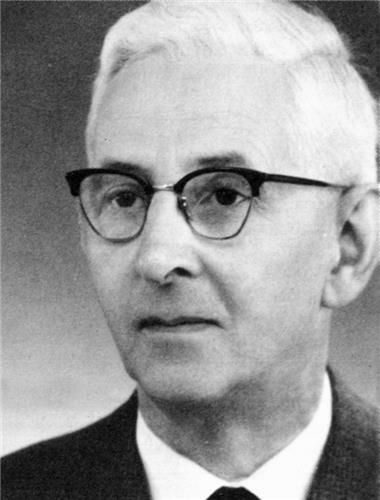
\includegraphics[height=.6\textheight]{../assets/Heyting}
    \end{column}
    \begin{column}{.7\textwidth}
      \begin{itemize}[<+->]
        \item Arend Heyting (1898--1980)
                
        \item Dutch logician, student of Brouwer
        
        \item Formalized intuitionistic logic
        
        \item e.g. `$\neg \phi$' means that there is a (computable) function that converts a proof of $\phi$ into a proof of a contradiction (e.g. $0=1$)
        
                   %  \item Rule-following paradox: relevant for interpreting Turing Machines, e.g. Church--Turing thesis. e.g. is anything an effective method or algorithmic? e.g. not requiring any creativity?
     
      \end{itemize}
    \end{column}
  \end{columns}
\end{frame}


\begin{frame}
\frametitle{Effectively Formalized Languages}
%\large

\begin{itemize}[<+->]

%\item A theory $T$ consists of an interpreted language $\mathcal{L}$ with a set of axioms and inference rules

\item An (interpreted) language $\mathcal{L}$ is \emph{effectively formalized} iff

\begin{enumerate}[1.)]

\item It has a finite set of basic symbols (recursion base)

\item There is an effective method for deciding whether any string of symbols written in $\mathcal{L}$ is a term/name, well-formed formula (wff), or a sentence.

\item There is an effective method for deciding whether any given sentence is true/false relative to an interpretation (e.g. an assignment of truth-values to basic symbols). 



\end{enumerate}

\item Example: first-order logic with identity 

\end{itemize}
\end{frame}

\begin{frame}
\frametitle{Effectively Axiomatized Theories}
%\large

\begin{itemize}[<+->]

\item A theory $T$ consists of an interpreted language $\mathcal{L}$ with a set of inference rules (proof system of a FOL) and (non-logical) axioms

\item \emph{Derivability}: a sentence $\phi$ is \emph{derivable/provable in $T$} iff there is a finite sequence of sentences, beginning with axioms and applying inference rules, that ends with $\phi$.

\item[] -- In this case we write ``$T \vdash \phi$" (read `$T$ proves (a.k.a. derives) $\phi$'; \\ where `$\vdash$' is called a `single turnstile')

\item \textbf{Effectively Axiomatized}: there exists effective methods both for deciding (i) whether a given sentence is an axiom and \\ (ii) whether a given array of wffs is a derivation. 


\end{itemize}
\end{frame}



\begin{frame}
\frametitle{Semantic vs. Syntactic notions}
%\large

\begin{itemize}[<+->]

\item \emphz{Semantic notions} involve truth, e.g. assigning truth values to sentences in an interpreted formal theory. \\ Truth is our simplified stand-in for \textcolor{OGlyallpink}{meaning}.
% Semantics is typically settled/presented by assigning ``semantic values to the basic non-logical expressions of the language, fix domains of quantification, and then give rules for working out the truth-conditions of longer and longer expressions in terms of the way they are syntactically built up from their parts" [smith,3)

\item \emph{Syntactic notions} are purely formal, without any interpretational content. A matter of what the theory can mechanically express. 
\item[] -- e.g. which strings of symbols constitute well-formed formulae and which of these are sentences (i.e. closed wffs with no unbound variables)
%settled by giving a finite recursion base of wffs and finite number of recursion clauses for building up larger wffs from these. 

\item We'll see that G\"odel's incompleteness theorem comes in these two varieties. The syntactic version is more troublesome for Hilbert's program.

\end{itemize}
\end{frame}


\begin{frame}
\frametitle{Syntactic (In)completeness}
%\large

\begin{itemize}[<+->]

\item On either variety, the relevant notion of incompleteness for G\"odel's theorem is syntactic rather than semantic:

\item A theory $T$ is \emph{negation complete} iff for every sentence $\phi \in \mathcal{L}$, either $T \vdash \phi$ or $T \vdash \neg \phi$ (i.e. T \textit{decides} every sentence in $\mathcal{L}$)

\item Notice that inconsistent theories are trivially negation complete, since they prove every sentence (in a classical logic, you can derive any sentence from a contradiction)

\item \textbf{Negation Incomplete}: there exists some $G$ in $T$'s language that $T$ does not decide, i.e. $T \nvdash G$ and $T \nvdash \neg G$

%so then by completeness of FOL, and assuming we've let $G$ be the true one of G or \neg G, we see that the axioms of T do not LOGICALLY entail G, i.e. $\Sigma \nentails G$. so this is unlike the `completeness' of FOL, where every logical truth is indeed proved by the system. 
%here we see there are arithmetic truths that are NOT proved by the system! 

\end{itemize}
\end{frame}

\begin{frame}
\frametitle{Semantic Completeness}
%\large

\begin{itemize}[<+->]

\item Semantic Completeness captures notion of logical entailment

\item Let $\Gamma$ be any set of \textit{sentences} of $\mathcal{L}$ and $\phi$ any sentence of $\mathcal{L}$. We work within a formally axiomatized theory $T$ with turnstile $\vdash_T$:

\item A first-order logical language comes equipped with a relation of \emphz{semantic entailment}, denoted by `$\entails$' (i.e. logical entailment):
\item[] $\Gamma \entails \phi$: $\phi$ is true on any interpretation that makes all sent. in $\Gamma$ true % makes $\phi$

\item \emphz{Semantic Completeness}: If $\Gamma \entails \phi$, then $\Gamma \vdash_{T} \phi$
%Double Turnstile entails  Single turnstile  

%\item By proving that QND is \textit{complete}, we show that 
%what about showing a set of sentences is unsatisfiable though? can we just not do this w/ SND derivations? would we need to introduce a falsum symbol? 

\medskip 

\bi

\item reasoning about arbitrary models/interpretations is not needed to demonstrate validity: derivations in $T$ suffice 

\item (logical entailment is fully covered by our syntactic rules)


\ei

\item First-order languages (including standard theories of arithmetic) are semantically complete, but NOT syntactically complete

\end{itemize}
\end{frame}

\begin{frame}
\frametitle{One Upshot of Negation Incompleteness}
%\large

\begin{itemize}[<+->]

\item Note the contrapositive of semantic completeness: \\ If $\Gamma \nvdash_{T} \Theta$, then $\Gamma \nentails \Theta$

\item Since any sufficiently strong arithmetical theory $T$ is (negation) incomplete, we know that there is a true G\"odel sentence $G$ that \\ $T$ does not decide, i.e. $T \nvdash_T G$.

\item So by the contrapositive of semantic completeness, \\ the axioms $\Sigma$ of $T$ do not \textit{logically} entail $G$: $\Sigma \nentails G$

\item So there is some countermodel of our arithmetical theory $T$ that makes its axioms true but that makes $G$ false

\item So the (quantified) arithmetical truths appear to outstrip those of logic (clearly an issue for the prospects of Logicism)

\item (In contrast, for any logical truth $\Theta$, we have $\entails \Theta$ and hence $\vdash_T \Theta$)
%it's in this sense that FOL is `complete': it formally decides all the logical truths
%but FOL is still UNDECIDABLE as a theory, in the sense that there is no effective method for spitting out these truths

%so we see arithmetic has formally undecidable sentences and so of course then is an undecidable theory. but see boolos/jeffrey discussion in ch. 17 about this...

\end{itemize}
\end{frame}

\begin{frame}
\frametitle{Soundness vs. Consistency}
%\large

\begin{itemize}[<+->]

\item Let $T$ be a formal axiomatized theory

\item $T$ is \emphz{sound} iff (i) its axioms are true and (ii) its proof system is truth-preserving (so all its theorems are true) \\

\item[] i.e. If $\Gamma \vdash_T \phi$, then $\Gamma \entails \phi$

\item[] -- Soundness is a \textcolor{OGlyallpink}{semantic} property

\item $T$ is \emph{consistent} iff there is no $\phi$ such that $T \vdash \phi$ and $T \vdash \neg \phi$

\item[] -- Consistency is a \textcolor{highlightA}{syntactic} property

\item[] -- Assuming mathematical reality is consistent, soundness implies consistency (so consistency is a weaker notion) 
% intuitively, syntax is weaker than semantics. Semantics involves specifying an interpretation., E.g. an interpretation of non-logical vocabulary.

\end{itemize}
\end{frame}


\iffalse %seems confusing to introduce this notion of soundness as well; going to stick w/ smith's convention instead 

\begin{frame}
\frametitle{Soundness and (Semantic) Completeness}
%\large

\begin{itemize}[<+->]

\item Let $\Gamma$ be any set of \textit{sentences} of $\mathcal{L}$ and $\phi$ any sentence of $\mathcal{L}$. We work within a formally axiomatized theory $T$ with turnstile $\vdash_T$:

\item A first-order logical language comes equipped with a relation of \emphz{semantic entailment}, denoted by `$\entails$' (i.e. logical entailment):
\item[] $\Gamma \entails \phi$: $\phi$ is true on any interpretation that makes the sentences $\Gamma$ true % makes $\phi$

%\item For our two natural deduction systems SND and QND, we have proven the following (where QND extends SND):

\medskip 

\item \emphz{Soundness}: If $\Gamma \vdash_T \phi$, then $\Gamma \entails \phi$
%Single turnstile entails Double Turnstile 

\bi 

\item Derivations in $T$ are `safe' (they preserve truth)

%\item (syntactic to semantic: i.e. we chose `good' rules!)

\ei

\bigskip 

\item \emphz{(Semantic) Completeness}: If $\Gamma \entails \phi$, then $\Gamma \vdash_{T} \phi$
%Double Turnstile entails  Single turnstile  

%\item By proving that QND is \textit{complete}, we show that 
%what about showing a set of sentences is unsatisfiable though? can we just not do this w/ SND derivations? would we need to introduce a falsum symbol? 

\medskip 

\bi

\item reasoning about arbitrary models/interpretations is not needed to demonstrate validity: derivations in $T$ suffice 

\item (logical entailment is fully covered by our syntactic rules)


\ei

\end{itemize}
\end{frame}


\fi %end of day two stuff  





\begin{frame}
\frametitle{G\"odel's First Incompleteness theorem(s)}
%\large

\begin{itemize}[<+->]

\item \emphz{Semantic Version}: suppose $T$ is a formal axiomatized theory containing the language $L$ of basic arithmetic. \\ If $T$ is \textcolor{OGlyallpink}{sound}, then $T$ is negation incomplete. i.e. there is a (\textcolor{OGlyallpink}{true}) sentence $G$ of $L$ such that $T \nvdash G$ and $T \nvdash \neg G$. 
%So $T$ is negation incomplete. 
% But if we reject the law of excluded middle, then we can infer that G is true. 

\item \emph{Syntactic Version}: suppose $T$ is a formal axiomatized theory containing the language $L$ of basic arithmetic. Then, if $T$ is \textcolor{highlightA}{consistent} and \textcolor{highlightA}{strong enough to prove} a fragment of arithmetic $Q$, then $T$ is negation incomplete.
%  i.e. there is a (\textcolor{OGlyallpink}{true}) sentence $G$ of $L$ such that $T \nvdash G$ and $T \nvdash \neg G$. 



\end{itemize}
\end{frame}

\subsection{Proof Sketch} 

\begin{frame}
\frametitle{Outline of Proof Idea}
%\large

\begin{enumerate}[<+->]

\item We choose a \textit{G\"odel-numbering scheme} for $T$: coding each (sequence of) wff(s) of $T$ as a unique natural number, \\ where our coding scheme provides an effective method %(algorithm)
% or more precisely, according to a primitively recursive method

\item Define predicates in $T$ that express the properties of coding for \\ (i) wff, (ii) sentences, and (iii) proofs in $T$
% these are numerical properties: they are properties of natural numbers in our coding scheme. So they are defined on our domain of quantification, which is the natural numbers.
% theorem: these properties/relations are effectively decidable

\item Show that $T$ can \textit{express} the proof-predicate \textrm{Prf(x, y)}, and hence the provable-in-$T$ predicate \textrm{Prov}$_T$(x) %$\mathsf{Prov_T(x)}$

\item Construct a G\"odel sentence $G$ that is true iff it is not provable, i.e. $G$ is true iff $\neg$\textrm{Prov}$_T$(g) is true, where $g$ codes for $G$

\item Show that if $T$ is sound, then $G$ is undecidable, and hence $T$ is negation incomplete, i.e. $T \nvdash G$ and $T \nvdash \neg G$.
% So there is some true sentence that the theory T does not decide

\end{enumerate}
\end{frame}

\begin{frame}
\frametitle{Philosophy Prompt \#23: G\"odel is NOT a liar!}
%\large

\begin{itemize}[<+->]

\item The proof of incompleteness relies on an arithmetic sentence $G$ that is \textit{true iff it is not provable} in a theory $T$ that contains enough arithmetic

\item This sentence functions like the claim ``I am unprovable in $T$"

\item This sentence might remind you of a \textbf{liar sentence}:\\ `` \textit{This sentence is not true}."
% True if and only if it is false, which is paradoxical

\item What should we say about the truth-value of the liar sentence? 
\item[] -- Should we be concerned that G\"odel's proof relies on a sentence that seems structurally similar to a liar sentence, since liar sentences lead to paradox?

% Crucial therapeutic remark: the formal theory $T$ can't also express the property of being a true sentence in $T $. This shows that the property of being a true T-sentence must be a different property than that of being a provable-in-T sentence. [See page 20 of Smith, without too many tears]
% proceed to section 16.5
% it still seems possible that a constructivist could deny that the true-in-T predicate does anything significant. e.g. just define `real truth' as what is co-extensional with the provable-in-T predicate. 

\end{itemize}
\end{frame}

\begin{frame}
\frametitle{Curry's (medieval) paradox (Prompt \#23 2.0)}
%\large

\begin{itemize}[<+->]

\item Consider $\phi$: `if this sentence is true, then Hunt is a millionaire'

\item Let $\psi$ stand for ``Hunt is a millionaire"

\item To all my 24.241 stans out there, this one goes out to you:
\vspace{-1em}
\end{itemize}
\pause
 \begin{columns}
    \begin{column}{.5\textwidth}
\footnotesize
\begin{fitchproof}
  \hypo{a}{\phi \eiff (\phi \eif \psi)} \pr{(By definition of $\phi$?)}%\pause
  \open
  \hypo{c}{\phi}\as{for conditional intro}\pause
  \have{d}{\phi \eif \psi}\by{Biconditional Elim}{a,c}\pause
  \have{g}{\psi}\ce{c, d}\pause
 \close
  \have{h}{\phi \eif \psi}\ci{c-g}\pause
  \have{i}{\phi}\be{a, h}\pause
  \have{j}{\psi}\ce{h, i}\pause 
\end{fitchproof}
    \end{column}

  \begin{column}{.6\textwidth}

\begin{itemize}[<+->]

\item So it appears that I'm a millionaire after all! 

\item[] -- one-boxing really pays the bills

\bigskip

\item What goes wrong in this argument?

\item[] (This curry's just too spicy)

%\item It seems like $\phi$ holds iff 

\end{itemize}
 \end{column}
 \end{columns}

\end{frame}

\begin{frame}
\frametitle{Resolutions of Curry's Paradox}
%\large

\begin{itemize}[<+->]

\item Recall $\phi$: `If this sentence is true, then Hunt is a millionaire'

\item[] we let $\psi$ stand for ``Hunt is a millionaire"

\item In our `proof', we assumed: $\phi \eiff (\phi \eif \psi)$

\item If $\phi$ stands for the whole conditional, then the antecedent should really be $True(\phi)$, so that we assume $\phi \eiff (True(\phi) \eif \psi)$

\item We then implicitly appealed to a disquotation principle $True(\alpha) \eiff \alpha$ to get to $\phi \eiff (\phi \eif \psi)$

\item So perhaps one of these steps is the culprit! 

\item e.g. perhaps we should deny that $True(\phi)$ is well-defined in our language 

\end{itemize}
\end{frame}

\begin{frame}
\frametitle{Expressing the Proof relation}
%\large

\begin{itemize}[<+->]

\item \emphz{Lemma 1}: let $T$ be a formal axiomatized theory containing the language $L$ of basic arithmetic. Suppose we have settled on a G\"odel-numbering scheme. Then $T$ can \textit{express} the proof relation $Prf$ using some wff \textrm{Prf(x,y)}: 

\item[] --i.e. \textrm{Prf(m, n)} is true iff $m$ codes for a proof-in-$T$ of the sentence with G\"odel number $n$
% notice how this is similar to coding a Turing machine that outputs the code of some function, i.e. computes a function. 

\item[] -- This is our G\"odelian analog of the lemma involving expressing the halting function

\end{itemize}
\end{frame}

\begin{frame}
\frametitle{Expressing a Provability predicate}
%\large

\begin{itemize}[<+->]

\item Using the predicate \textrm{Prf(x,y)}, it is easy to express the claim that a number codes a sentence that has a proof-in-$T$:

\item Define \textrm{Prov(x)} $:=$ $\exists$\textrm{z Prf(z, x)}, i.e. \textrm{Prov(n)} is true iff some number $m \in \mathbb{N}$ codes a $T$-proof of sentence with G\"odel number $n$

%\item Diagonal argument: 
\item Now consider a sentence that is true iff it is not provable!
%i.e. a sentence that is true iff it is not a theorem of T

\item \emphz{Lemma 2}: We can construct a G\"odel sentence $G$ in the language $L$ such that $G$ is true iff $\neg$\textrm{Prov}$_T$(g) is true, where $g$ is the code number for $G$.  



\end{itemize}
\end{frame}


\iffalse 
\begin{frame}
\frametitle{G\"odel Sentence}
%\large

\begin{itemize}[<+->]

\item Lemma 2: We can construct a G\"odel sentence $G$ in the language $L$ such that $G$ is true iff $\neg$\textrm{Prov}$_T$(g) is true, where $g$ is the code number for $G$ 

\end{itemize}
\end{frame}
\fi 

\begin{frame}
\frametitle{Proving Incompleteness (semantic version)}
%\large

\begin{itemize}[<+->]

\item Let $T$ be a \textcolor{OGlyallpink}{sound} formal axiomatized theory that can express a predicate \textrm{Prf(x,y,)}. Lemma 2 provides a G\"odel sentence $G$. 

\item[] -- Assume for \textit{reductio} that $T \vdash G$. 
\item[] -- By construction, $G$ is true iff it is not provable. 
\item[] -- So $T \vdash G$ $\Rightarrow$ $G$ is false. 
\item[] -- But then $T$ would prove a false sentence, so it would not be sound (contradiction). Hence $T \nvdash G$, so $G$ is not provable

\item Hence, by construction, $G$ is true, so $\neg G$ is false.
\item[] -- Since $T$ is sound, it cannot prove anything false, so $T \nvdash \neg G$

\item So $T$ is negation incomplete!

\end{itemize}
\end{frame}


\subsection{Background from FOL}

\begin{frame}
\frametitle{Soundness and Completeness of FOL}
%\large

\begin{itemize}%[<+->]

\item Let $\Gamma$ be any set of \textit{sentences} of QL and $\Theta$ any sentence of QL. 

\item For our two natural deduction systems SND and QND, we have proven the following (where QND extends SND):

\medskip 

\item \emph{Soundness}: If $\Gamma \vdash_{QND} \Theta$, then $\Gamma \entails \Theta$
%Single turnstile entails Double Turnstile 

\bi 

\item QND derivations are `safe' (they preserve truth)

\item (syntactic to semantic: i.e. we chose `good' rules!)

\ei

\bigskip 

\item \emph{Completeness}: If $\Gamma \entails \Theta$, then $\Gamma \vdash_{QND} \Theta$
%Double Turnstile entails  Single turnstile  

%\item By proving that QND is \textit{complete}, we show that 
%what about showing a set of sentences is unsatisfiable though? can we just not do this w/ SND derivations? would we need to introduce a falsum symbol? 

\medskip 

\bi

\item reasoning about arbitrary models is not needed to demonstrate validity: QND derivations suffice

\item (logical entailment is fully covered by our syntactic rules)


\ei

\end{itemize}
\end{frame}


\begin{frame}
\frametitle{\metav{L}-models and interpretations}
%\large

\begin{itemize}%[<+->]

\item Let \metav{L} be a first-order language, containing constants and $k$-place predicates (e.g. the language of QL)
\bi
\item recall that the atomic sentences of SL are 0th-place predicates
\ei
\item An \metav{L}-model $\mathfrak{M} := (D, I)$ consists of

\begin{enumerate}

\item A non-empty set $D$ of objects, called the domain of   $\mathfrak{M}$

\item A map I (the \textit{interpretation} of $\mathfrak{M}$), which maps the vocabulary of \metav{L} to objects and ordered pairs from $D$ as follows:

\begin{itemize}

\small

\item For each constant $c \in \mathfrak{L}$, $I(c)$ is an element of $D$, called the \textit{referent} or denotation of $c$

\item For each k-place predicate $P$ of $\mathfrak{L}$, $I(P)$ is a set of ordered $k$-tuples of objects in $D$, called the \textit{extension} of $P$
\item $I$ maps SL atomics to ``true" or ``false" (i.e. `1' or `0')
% $k$-place relation defined on $D$, 
% GB: you can think of a k-place relation as a subset of $D^k$, i.e. the space of k-tuples of objects in D. 

\end{itemize}

\end{enumerate}

%\item Our text uses `models' and `interpretations' interchangeably, but the above disambiguation is convenient

\end{itemize}
\end{frame}

\begin{frame}
\frametitle{Decidability of Propositional and Monadic Predicate Logic}
%\large

% % From Gordon Belot logic 303 notes, 28: The Undecidability of Predicate Logic 

\begin{itemize}[<+->]

\item A logic is \emph{decidable} if there is an effective method that determines whether or not an arbitrary wff $\phi$ is a logical truth, i.e. settles whether $\phi$ is a theorem (i.e. whether $\entails \phi$)

\item Sentential/propositional logic is decidable: truth tables provide an effective method

\item Monadic predicate logic is decidable: you can convert a question about the logical truth of a formula $\phi$ with $k$ one-place predicates into a question about whether it is true in all models with $2^k$ or fewer objects, and convert this question into one that a truth-table can settle


\end{itemize}
\end{frame}


\begin{frame}
\frametitle{Undecidability of First-order Logic}
%\large

\begin{itemize}[<+->]

\item Once we add in two-place predicates and beyond, matters become more complex: 
% both church and touring proved this, independently, in 1936

\item  \emphz{Church's Theorem}: first-order logic is undecidable, i.e. there is no effective method to determine the set of logically-valid sentences

\item Note that we can code wffs of FOL with identity as numbers

\item Turing's statement of this theorem: there is no Turing machine that takes as input the code number of an arbitrary wff $\phi$ and always halts, giving output $1$ iff $\phi$ is a logical truth

\item Notice how similar this statement is to our Version$_1$ of the incompleteness of \textit{arithmetic} 

\end{itemize}
\end{frame}

\begin{frame}
\frametitle{Sentence Decidability and (Negation) Completeness}
%\large

\begin{itemize}[<+->]

\item If $T$ is a theory and $\phi$ is a sentence in $T$'s language, then $T$ \emph{formally decides} $\phi$ iff either $T \vdash \phi$ or $T \vdash \neg \phi$

\item So a sentence $\phi$ is \emphz{formally undecidable} by $T$ iff $T$ doesn't decide it, i.e. $T \nvdash \phi$ or $T \nvdash \neg \phi$

\item A theory $T$ is \emph{negation complete} iff it formally decides every sentence of its language, i.e. for every $\phi$, either $T \vdash \phi$ or $T \vdash \neg \phi$

\item So to say that a theory is \emphz{negation incomplete} is just to say that there is some formally undecidable sentence of $T$, i.e. some sentence $G$ that $T$ does not settle

%\item Notice that undecidability \textit{of a theory} does NOT entail being semantically incomplete, e.g. FOL is undecidable but semantically incomplete
%% but is FOL negation complete? seemingly not. it seems negation complete only with respect to the logical truths. but not all wffs are either a tautology or a contradiction. and FOL doesn't decide these, i take it? try to figure this out. 

% %Question: does semantically complete for logical truths entail negation complete? 
% not sure if this is true...\item Notice that FOL is semantically complete and hence negation complete but \textit{undecidable} in a different sense!

%clearly this is different from the THEORY being undecidable. e.g. since 

\end{itemize}
\end{frame}



%\fi %end of day 2 stuff *********************************************************

\subsection{Incompletability}

\begin{frame}
\frametitle{G\"odel's First Incompleteness theorem(s)}
%\large

Recall from last time:

\begin{itemize}[<+->]

\item \emphz{Semantic Version}: suppose $T$ is a formal axiomatized theory containing the language $L$ of basic arithmetic. \\ If $T$ is \textcolor{OGlyallpink}{sound}, then $T$ is negation incomplete. i.e. there is a (\textcolor{OGlyallpink}{true}) sentence $G$ of $L$ such that $T \nvdash G$ and $T \nvdash \neg G$. 
%So $T$ is negation incomplete. 
% But if we reject the law of excluded middle, then we can infer that G is true. 

\item \emph{Syntactic Version}: suppose $T$ is a formal axiomatized theory containing the language $L$ of basic arithmetic. Then, if $T$ is \textcolor{highlightA}{consistent} and \textcolor{highlightA}{strong enough to prove} a fragment of arithmetic $Q$, then $T$ is negation incomplete.
%  i.e. there is a (\textcolor{OGlyallpink}{true}) sentence $G$ of $L$ such that $T \nvdash G$ and $T \nvdash \neg G$. 

\item Could we simply supplement $T$ (e.g. $\mathsf{PA}$) to fix incompleteness?

\end{itemize}
\end{frame}

\begin{frame}
\frametitle{Mo' axiom\$\$\$, Mo' problems}
%\large

\begin{itemize}[<+->]

\item Picture this: you are confronted with a G\"odel sentence $G $ that your theory $T$ does not decide. What do you do?

\item You could add $G$ as an axiom, resulting in $T^+$. Then since $G \vdash G$, we'd have $T^+ \vdash G$. 

\item Or maybe you think there's a family of undecidable $G$s that an axiom (or a couple) added to $T$ would resolve. 

\item Bad news: any formally axiomatized, sufficiently strong arithmetical theory $T$ is negation incomplete, no matter how many axioms we add :( 

\end{itemize}
\end{frame}

\begin{frame}
\frametitle{Incompletability}
%\large

\begin{itemize}[<+->]

\item On both the syntactic and semantic versions of G\"odel's incompleteness theorem, the construction of a G\"odel sentence $G$ generalizes to any strengthening of $T$ with new axioms:

\item On the semantic version, $G$ is true (as we argued), so adding it to $T$ preserves soundness (true axioms and truth preserving deductions)

\item On the syntactic version, $T \nvdash \neg G$, so $G$ is consistent with $T$ (\& assuming law of excluded middle, we can argue that $G$ is true)

\item So adding the G\"odel sentence of $T$ to form $T^+$, we can simply construct a new G\"odel sentence for $T^+$, and so on.

\item in other words: ``IT NEVER ENDS"! 
%\item[] -- 
\item[] \footnotesize{(unless we either (i) give up on having an effectively axiomatized theory \\ or (ii) give up on having a language as rich as $L$, \\ or (iii) give up on proving at least as much arithmetic as $\mathsf{Q}$)}

\end{itemize}
\end{frame}

%\subsection{Philosophical Ramifications} 

\subsection{Sources of Incompleteness}

\begin{frame}
\frametitle{Peano Arithmetic ($\mathsf{PA}$) vs. Robinson Arithmetic ($\mathsf{Q})$}
%\large

\begin{itemize}[<+->]

\item A theory $\mathsf{PA}$ with language $L=\langle 0, +, \times, S\rangle$, here using successor function rather than the constant $1$, equipped with a proof system, six non-logical axioms, and an induction schema:

\begin{enumerate}[1.)]

\item $\mathsf{\forall x \neg(0 = Sx)}$

\item $\mathsf{\forall x \forall y (Sx = Sy \eif x = y)}$

\item $\mathsf{\forall x (x + 0 = x)}$

\item $\mathsf{\forall x \forall y (x + Sy = S (x + y))}$

\item $\mathsf{\forall x (x \times 0 = 0)}$

\item $\mathsf{\forall x \forall y (x \times Sy = (x \times y) + x)}$

\end{enumerate}


\item[] \textbf{Induction Schema}: $\mathsf{\big (\phi(0) \eand \forall x (\phi(x) \eif \phi (Sx)) \big) \eif \forall x \phi (x)}$ \\ where $\phi(x)$ is an arbitrary open wff of $L$ 

\item $\mathsf{Q}$ is $\mathsf{PA}$ minus the induction schema, plus an axiom stating that every number except zero is a successor: $\mathsf{ \forall x (x \neq 0 \eif \exists y (x = Sy) ) }$
%in PA we can derive this axiom, e.g. see p. 44 of smith, WTmTears
%what we get leaving out

%part of interest of Q is that it, unlike PA, has finitely-many axioms. so it shows that the issue is not having infinitely many axioms. 

%from wiki on raphael robinson: ``In 1950 Robinson proved that an essentially undecidable theory need not have an infinite number of axioms by coming up with a counterexample: Robinson arithmetic Q. Q is finitely axiomatizable because it lacks Peano arithmetic's axiom schema of induction; nevertheless Q, like Peano arithmetic, is incomplete and undecidable in the sense of Gödel. "

%other e.g.s of undecidable theories: ``Robinson's work on undecidability culminated in his coauthoring Tarski et al. (1953), which established, among other things, the undecidability of group theory, lattice theory, abstract projective geometry, and closure algebras."


\end{itemize}
\end{frame}

\begin{frame}
\frametitle{Incompleteness of Robinson arithmetic $\mathsf{Q}$}
%\large

\begin{itemize}[<+->]

\item $\mathsf{Q}$ is incomplete in a much more boring way than $\mathsf{PA}$ % Peano Arithmetic!

\item It can't prove an obviously true universal generalization, namely that $0$ is an additive identity: $\mathsf{\forall x (0+x = x)}$. Denote this by `$\phi$' 
%see page 36-37 of smith, without too many tears
%notice how surprising this result is is, given the similarity to Axiom 3 above! Q can prove any particular instance of 0 + n = n (for the regular naturals), but not the universal generalization, since we can have a domain of discourse with deviant non-standard elements a and b, such that 0+a = b and 0 +b = a. 

\item From soundness of first-order logic, If $\mathsf{Q} \vdash \phi$, then $\mathsf{Q} \entails \phi$. \\ Contrapositive: if $\mathsf{Q} \nentails \phi$, then $\mathsf{Q} \nvdash \phi$

\item S to prove $\mathsf{Q} \nvdash \phi$, suffices to construct a countermodel to $\mathsf{Q} \entails \phi$, i.e. a model where all the axioms of $\mathsf{Q}$ are true but $\phi$ is false 

\item[] $\Rightarrow$ $\exists$ arithmetical truths not \textit{logically} entailed by $\mathsf{Q}$'s axioms

\item Since $\mathsf{Q}$ is sound, it can't prove $\neg \phi$ either 

\item So $\mathsf{Q}$ doesn't decide $\phi$, making it negation incomplete 

\item $\mathsf{Q}$ shows that even a \textit{finitely}-axiomatized theory can be incomplete 

\end{itemize}
\end{frame}

\begin{frame}
\frametitle{Quantifier-Free}
%\large

\begin{itemize}[<+->]

\item If we leave out the quantifier $\forall$ from $L$, we can construct an effectively axiomatized theory that is negation complete

\item[] -- So the quantifier-free fragment of elementary arithmetic is negation complete

\item Unsurprisingly, Robinson arithmetic decides every quantifier-free sentence of $L$

\item So is the source of incompleteness adding quantifiers?

\end{itemize}
\end{frame}

\begin{frame}
\frametitle{Are Quantifiers to Blame?}
%\large

\begin{itemize}[<+->]

\item No!

\item Elementary Euclidean geometry can be captured in a consistent, negation complete, and decidable first-order theory (Tarski 1959)
%not sure if Tarski proved all these results in 1959, vs some of them being proved later? 

\item Tarski's axiomatization is first order, with quantifiers $\forall$ and $\exists$

\item Primitive predicates for between \& congruent (same length), \\ 10 axioms and an axiom schema (so countable infinity of axioms)
% domain of discourse is simply points (no lines). First-order logic with identity 

\item So quantifiers do not necessarily lead to incompleteness

\item (One can't capture $\mathsf{Q}$ in Euclidean geometry; otherwise, it \textit{would} be negation incomplete)


\end{itemize}
\end{frame}


\subsubsection{That's one complete Burger}
%one burger please; a burger with the works 

\begin{frame}
\frametitle{Presburger Arithmetic}
%\large

\begin{itemize}[<+->]

\item Define $\mathsf{P}$ as the fragment of Peano Arithmetic that drops the multiplication function $\times$ and its associated two axioms %for multiplication

\item Theorem (1929): Presburger Arithmetic is negation complete
% the proof is provided in bolos/Jeffrey chapter 24, using the method of quantifier elimination. Basic idea seems to be the following: for any claim in arithmetic using just addition and successor, you can always find a coextensive claim that does not involve quantifiers. And the quantifier-free fragment of arithmetic is negation complete (as is shown with Baby Arithmetic).

\item Question: but isn't multiplication simply repeated applications of addition? 
\item[] -- So why can't we simply \textit{define} or \textit{express} multiplication within $\mathsf{P}$ , e.g. in the way that we introduce other predicates like \textrm{Prf(x, y)} using the primitives of language $L$? 

\end{itemize}
\end{frame}

\begin{frame}
\frametitle{The Existence of Recursively Defined Functions}
%\large

\begin{itemize}[<+->]

\item Notice that within PA, we introduce multiplication recursively, using two axioms:
\item[] $\mathsf{\forall x (x \times 0 = 0)}$ and $\mathsf{\forall x \forall y (x \times Sy = (x \, \textcolor{highlightA}{\boldsymbol{\times}} \, y) + x)}$
\item[] -- Notice that `$\boldsymbol{\textcolor{highlightA}{\times}}$' still appears on RHS! We haven't eliminated it. 
%still appears on the RHS! We haven't formally eliminated it. 

\item Short of (i) equipping a theory with function $\times$ \& these two axioms \\ or (ii) working within set theory, we can't prove that a unique multiplication function exists 
\item[] (in set theory one can prove a Recursion Theorem stating that recursively defined functions exist and are unique). 

\item So Presburger Arithmetic can't recover multiplication, atlhough of course $\mathsf{P}$ can express repeated applications of addition, like $4 + 4 + 4$, which intuitively matches $4 \times 3$ but is technically not the same function. 

\end{itemize}
\end{frame}

\begin{frame}
\frametitle{vs. Expressing non-basic Predicates/Functions}
%\large

\begin{itemize}[<+->]

\item In contrast, one \textit{can} properly define exponentiation in terms of addition and multiplication

\item Similarly, one can define addition in terms of successor and multiplication:

\item[] $\mathsf{x + y = z}$ holds if and only if the following equation holds: \\ 
\footnotesize{$\mathsf{S(Sx\times SSz)\times S(Sy \times SSz) = S( ( S( Sx \times Sy) \times (SSz \times SSz)))}$}


%\footnotesize{$\mathsf{S(S(x)\times SS(z))\times S(S(y) \times SS(z)) = S( ( S( S(x) \times S(y)) \times (SS(z) \times SS(z))))}$}

\item[] e.g. $1+2 = 3$: $\mathsf{S(2 \times 5) \times S (3 \times 5) = S ( S (2 \times 3) \times (5 \times 5))}$, \\ yielding $\mathsf{11 \times S(15) = S (7 \times 25) = 176}$

\item So the multiplicative analog of Presburger arithmetic (known as Skolem arithmetic) has just multiplication but no successor function. It is also negation complete. 

\end{itemize}
\end{frame}

\begin{frame}
\frametitle{The Source of Incompleteness?}
%\large

\begin{itemize}[<+->]

\item So FOLs with $\langle 0, S, + \rangle$ and $\langle 0, \times \rangle$ are both complete/decidable

\item[] -- Also non-FOL theories with $\langle 0, S, +, \times \rangle$ but no quantifiers

\item What goes `wrong' when we combine successor, addition, multiplication, and quantifiers?

\item We arrive at a theory $\mathsf{Q}$ (in language $L$) that is powerful enough to express any (primitively) recursive function. 

\item So at this point we can express predicates like $\mathsf{Prf (x, y)}$ and $\mathsf{Halt (x)}$, and as we've seen that's enough for incompleteness 

\item Metaphor: we see a kind of `phase transition' in the complexity of the sentences we can express 
%\textrm{Q} 
\end{itemize}
\end{frame}


\subsection{Whither Logicism?}
%\subsection{What's good, Logicism?} 


\begin{frame}
\frametitle{Logicism}
%\large

\begin{itemize}[<+->]

\item Recall logicism: all mathematical truths are \textit{analytic}: entailed by logic and axioms that are true-by-definition 
\item[] Slogan: math is logic plus definitions 

\item After destroying Frege's hopes and dreams, Russell remained confident in the logicist project, writing in 1903:

\pause 
\begin{quotation}
All mathematics deals exclusively with concepts definable in terms of a very small number of logical concepts, and \dots all its propositions are deducible from a very small number of fundamental logical principles.
\end{quotation}
% quoted by Smith on page 9, without too many tears

% Russell then tried to make good on this promise in the three volumes of the Principia, with Whitehead. And indeed, G\"odel is responding to the Principia, showing that there are undecidable propositions within this system.
% As Smith notes, we might already have issues with the axioms of Principia, which don't seem to simply be logical in nature, e.g. the axiom of infinity, and the axiom of reducibility
%  G\"odel incompleteness results show that even if we tried to clean up these aspects of Principia, we are destined to have undecidable propositions within a sufficiently strong arithmetic. And clearly, to capture all arithmetical truths, we need the system to at least be sufficiently strong.

\item G\"odel's incompleteness theorems throw a serious wrench in logicist ambitions: (classical) mathematical truth outstrips what we can (effectively) derive within systems that contain a modest amount of arithmetic
% and if our goal is to derive all of mathematics, then we of course need to derive all of arithmetic, so we at least need to derive this modest amount.

\end{itemize}
\end{frame}

\begin{frame}
\frametitle{A Logicist Retreat?}
%\large

\begin{itemize}[<+->]

\item Fragments of Peano Arithmetic are sound \& negation complete

\item \emph{Baby Arithmetic} ($\mathsf{BA}$): remove quantifiers from the language $L$, and replace six axioms of $\mathsf{PA}$ with schemas like $\mathsf{\zeta + S\xi = S(\zeta +\xi)}$ (so a countable-infinity of axioms)
%so we rely on quantifiers only in our meta-language, to talk about being allowed to instantiate every instance of each of these schemas, for our domain of natural numbers  
% as Smith page 31 (without too many tears) notes, ``although BA isn't finitely axiomatized, it is still an effectively axiomatized theory: given a candidate wff, we can effectively decide whether it is an instance of one of those six schemas and hence an axiom"

\item Clearly, the truths of $\mathsf{BA}$ capture a lot of the standard interpretation/meaning of arithmetic (all non-quantified truths concerning addition and multiplication)

\item So seemingly everyone can be a logicist at least about the arithmetic truths proved by $\mathsf{BA}$ \\ (regarding these as truths of logic-plus-definitions)
% see footnote 3 of Smith, page 34, without too many tears (he makes exactly this point, which I am copying basically verbatim)

\item But then what should we say about all the quantified truths of arithmetic? e.g. that $\mathsf{\forall x (x \times 0 = 0)}$

%\item So could the logicist take these truths to be partly constitutive of arithmetic?
\end{itemize}
\end{frame}

\begin{frame}
\frametitle{A Logicist Offensive? Going 2nd-order}
%\large

\begin{itemize}[<+->]

\item Alternatively, a logicist might appeal to second-order Peano Arithmetic ($\mathsf{PA_2} $)

\item Unlike 1st-order $\mathsf{PA} $, $\mathsf{PA_2} $ is \textit{categorical}: it has no non-standard models (all models of $\mathsf{PA_2} $ are isomorphic)

\item So there is a sense in which $\mathsf{PA_2} $ \textit{settles} all of the arithmetical truths of our language $L$ (in its intended interpretation)

\item Since $\mathsf{PA_2} $ contains $\mathsf{Q} $, it remains negation incomplete \\ (it will have its own canonical, undecidable G\"odel sentence)

\item Nonetheless, with second-order logical entailment $\entails_2$, \\ $\mathsf{PA_2} $ \textit{semantically entails} every truth of $L$
\item[] -- Gotta catch 'em all 

\end{itemize}
\end{frame}

\begin{frame}
\frametitle{What is happening$_{\text{what is happening}}$?}
%\large

\begin{itemize}[<+->]

\item Consider a G\"odel sentence $G_2$ of $\mathsf{PA_2} $, so $\mathsf{PA_2} \nvdash G_2$ and $\mathsf{PA_2} \nvdash \neg G_2$ 
\item[] As before, we can argue in our meta-language that $G_2$ is true in the standard interpretation of $L$. 

\item So the axioms $\Sigma_2$ of $\mathsf{PA_2}$ semantically entail $G_2$: $\Sigma_2 \entails_2 G_2$.

\item So clearly, $\mathsf{PA_2}$'s proof system is semantically incomplete, i.e. it's NOT the case that If $\Sigma_2 \entails_2 G_2$, then $\Sigma_2 \vdash_2 G_2$
\item[] -- and we can't do any better (lest we violate G\"odel's theorem)
%(provided we remain consistent and effectively axiomatized)
%

\item Whereas $\mathsf{PA}$ (as a first-order language) has a semantically complete proof system: if $\phi$ follows \textit{logically} from its axioms, we'll be able to derive $\phi$ in $\mathsf{PA}$. 

\end{itemize}
\end{frame}


\begin{frame}
\frametitle{But it's gonna cost you $\mathbb{R}$\$\$}
%\large
%What Price 2nd-order Arithmetic?

\begin{itemize}[<+->]

\item In any 2nd-order logic, we are permitted to `quantify over properties', e.g. $\mathsf{\forall X (\forall y X y \eif X 0)}$

\item In 1st-order logic, `properties' are defined as subsets of the domain of quantification, i.e. the \textit{extension} of a predicate is just the members of the domain that satisfy the predicate 

\item So in 2nd-order logic, we quantify over subsets of the domain

\item To end up with a categorical 2nd-order PA, we have to permit quantification over all arbitrary subsets of  $\mathbb{N}$: i.e. $\mathcal{P}(\mathbb{N})$
\item[] -- we won't in general have recipes for specifying the members of arbitrary infinite subsets

%\item Quantifies over arbitrary subsets of $\mathbb{N}$: i.e. $\mathcal{P}(\mathbb{N})$

\item So $\mathsf{PA_2}$ goes beyond `purely arithmetical' notions (which are always countable) into analysis (the continuum)

%\item So commits us to something like axiom of choice

\end{itemize}
\end{frame}

\begin{frame}
\frametitle{Axiom (Schemas) for $\mathsf{PA_2}$ }
%\large

\begin{itemize}[<+->]

\item Like $\mathsf{PA}$, $\mathsf{PA_2}$ remains effectively axiomatized:

\item[a.)] non-logical axioms of $\mathsf{Q}$

\item[b.)]  2nd-order Induction Schema: $\mathsf{\forall X ((X0 \eand \forall y (Xy \eif X Sy)) \eif \forall y X y)}$

\item[c.)] (Unrestricted) Comprehension Schema: $\mathsf{\exists X \forall y (Xy \eiff \phi(y))}$, \\ where $\phi$ is ANY predicate not containing $\mathsf{X}$ free
%the ANY predicate part is the unrestricted part. in principle we could restrict the comprehension schema to some (decidable) class C of wffs. see p. 210 of smith 
% technically taking the closure of every instance of this comprehension schema (but can't remember what exactly that means).

\item Hold-on! Won't this lead to a Russell's paradox infecting $\mathsf{PA_2}$?

\item Response: impredicative definitions are non-vicious if the class we're talking about exists independently of our definition
\item[] -- e.g. ``the tallest student in this room"; ``the least upper bound"


\end{itemize}
\end{frame}

\begin{frame}
\frametitle{G\"odel on Impredicative Definitions}
%\large

\begin{itemize}[<+->]

\item G\"odel (1933): just assume that ``the totality of all properties [of numbers] exists somehow independently of our knowledge and our definitions, and that our definitions merely serve to pick out certain of these previously existing properties"

\item This interpretation accords with how we are already interpreting second-order quantification in $\mathsf{PA_2}$, namely that the totality of all properties of numbers is fixed, namely by the extensions of predicates, comprising ALL the arbitrary subsets of $\mathbb{N}$

\item So this pretty much sounds like Platonism? But a logicist can be happy with that! After all, they've still gotten what they came for, namely the truths of arithmetic from `logic' and definitions alone \\ (and picked up a lot of analysis for free!) % On the side
% Still gotten a lot of what they wanted

\end{itemize}
\end{frame}


\iffalse % bad framing in the following slide, since technically second-order Peano arithmetic is still effectively axiomatized. You simply give up on having a semantically complete proof system

\begin{frame}
\frametitle{A Logicist Offensive? Going non-effective}
%\large

%read smith chapter on this in the big book 

\begin{itemize}[<+->]

\item Alternatively, could a logicist be in favor of rejecting the requirement of having an effectively axiomatized theory? 

\item Neo-logicists today work within second-order logic, constructing a system that \textit{semantically} entails all arithmetical truths
%Frege's theorem 

\item But there is no semantically complete proof system for second-order logic: so neo-logicists acknowledge that we can't capture this semantic entailment relation in a single effectively axiomatized theory 

\end{itemize}
\end{frame}

\fi 

\begin{frame}
\frametitle{Philosophy Prompt \#24}
%\large

\begin{itemize}[<+->]

\item What do you think that G\"odel's incompleteness theorem(s) tell us about the nature of mathematics or mathematical truth?

\item[] -- Do they provide evidence for mathematical Platonism?
% Do they weaken the plausibility of logicism, or formalism?
% Do they leave intuitionism or mathematical constructivism untouched?

\item More generally, has anything in this class changed how you think about the nature of mathematics?

\end{itemize}
\end{frame}


\begin{frame}
\frametitle{Logicism today: Neo!}
%\large

\begin{itemize}%[<+->]

\item \emph{Neo-logicism}: (i) we can know many mathematical truths \\ \textit{a priori}, deriving them from rules that are analytic or meaning-constitutive of the relevant mathematical concepts \\ (e.g. the concept \textsc{Number}) 
\item[] (ii) realism in ontology: objective, mind-independent mathematical objects exist
% % advantage of the root through logicism is to avoid some epistemic problems for Platonism otherwise construed. Mathematics becomes knowable a priori. We do not need causal connection with these abstract objects. We also do not need to appeal to some mysterious notion of intuition.

\item Using Hume's principle and second-order logic, one can derive the natural numbers and arithmetic (``Frege's theorem")
% % where Frege's original program goes wrong is that he aims to derive Hume's principle using the concept of extensions and the inconsistent Basic Law V. So Wright and Hale basically argue that they can recover Frege's program simply by starting with Hume's principle and second-order logic
% Shapiro notes that Hume's principle is consistent if (second-order) arithmetic is consistent.

\item Whether this shows arithmetic is epistemically closer to `logic' than `mathematics' depends on the status of 2nd-order logic

\item Quine: second-order logic is just disguised set theory \\ (`a wolf in sheep's clothing')
% C Quine 1986, philosophy of logic, second edition. Quoted by Schapiro on page 136. See especially chapter 5 of Quine.

%as Rayo notes in Topic 10 videos, we can prove the consistency of arithmetic within set theory, but the proof relies on axioms that we should be less secure about than we are about the arithmetical axioms. so maybe the idea here is similar! we shouldn't be necessarily secure about second-order logic and its consistency. 

\end{itemize}
\end{frame}



\subsection{\phantom{v} Tarski Serum}

\begin{frame}
\frametitle{Tarski's Theorem$_1$ (undefinability of truth in $T$)}
%\large

\begin{itemize}[<+->]

%\item Just like with provability, 

\item We attempt to define a predicate \textrm{True(n)} that is true iff $n$ is the G\"odel number of a true sentence in $T$ 
\item[] -- We allow that we might have to extend language $\mathcal{L}$ to some $\mathcal{L}^{\ast}$

\item \textbf{Truth-predicate}: \textrm{T(x)} is a truth-predicate for $\mathcal{L}$ iff `\textrm{T}($\overline{\phi}$) $\eiff \phi$' is true for every sentence $\phi$
\item[] Motivation: `snow is white' is true iff snow is white 
%provable for every sentence $\phi$

\item \emph{Tarski's theorem$_1$}: no consistent, effectively axiomatized theory $T$ which contains enough arithmetic (e.g. $Q$) can define truth for its own language, i.e. prove that `\textrm{T}($\overline{\phi}$) $\eiff \phi$' for every $\phi$. 

\item \textit{Upshot}: when we define truth within such theories, we must do so within a metalanguage. 

\end{itemize}
\end{frame}

\begin{frame}
\frametitle{Tarski's Theorem$_2$ (inexpressibility)}
%\large

\begin{itemize}[<+->]

\item We can't \textit{define} truth within $T$; can we at least \textit{express} truth in $T$?

\item \emph{Tarski's theorem$_2$}: no predicate within our arithmetic language $L$ can express the truth-predicate \textrm{True(n)}, i.e. the property of numbering a truth of $L$

\item In contrast, recall that we \textit{can} express a provability predicate in $L$

\item One upshot: there is a crucial difference between syntactic vs. semantic properties of languages that contain enough arithmetic

\item Moreover, we see immediately that the property of provability must be distinct from the property of being true
\item[] -- and that is essentially the (semantic) incompleteness result! 

\end{itemize}
\end{frame}

\begin{frame}
\frametitle{G\"odel's interpretation of Tarski's result}
%\large

\begin{itemize}[<+->]

\item G\"odel ultimately took Tarski's theorem to provide the underlying \textit{reason} for the incompleteness of arithmetic: 

\medskip 

\pause

\begin{quotation}

A complete epistemological description of a language $A$ cannot be given in the same language $A$, because the concept of truth of sentences in $A$ cannot be defined in $A$. It is this theorem which is the true reason for the existence of undecidable propositions in the formal systems containing arithmetic -- G\"odel in a letter
\end{quotation}
%see page 114, section 16.5 of smith, without too many tears


\item G\"odel took his incompleteness theorems as evidence for mathematical Platonism: mathematical truths obtain independently of mathematical agents

\end{itemize}


\end{frame}

% I suppose that in a course on paradoxes, it could be fun to discuss Curry's paradox. See page 112 of Smith, without too many tears.

%Curry's paradox could be a fun Philosophy Prompt, rather than having them reflect on the Liar's paradox! e.g. ask them to diagnose what has gone wrong in the Curry's paradox argument 


\begin{frame}
\frametitle{What can a Constructivist or non-Platonist say?}
%\large

\begin{itemize}[<+->]

%\item G\"odel took his incompleteness theorems as evidence for mathematical Platonism: mathematical truths obtain independently of mathematical agents

\item What might a non-Platonist say in response?

\item Constructivist: reject unrestricted law of excluded middle $p \eor \neg p$
\item[] -- restrict mathematical truth to what can be proved within an effectively axiomatized system
% % think about whether this interpretation is even consistent with the canonical G\"odel sentence.

\item Formally undecidable sentences are only true or false relative to consistent extensions, e.g. where they've been added as axioms

\item[] -- like how we can add a G\"odel sentence to $\mathsf{PA}$

\item Analogy: the parallel postulate is not true or false \textit{tout court} but only relative to a choice of geometry

\item[] -- likewise, many arithmetical sentences are only true/false relative to a choice of a model of arithmetic 

\end{itemize}
\end{frame}






 \iffalse %commenting out as bonus material

\subsection{\phantom{v} Frege and Neo-Logicism} 

\begin{frame}
\frametitle{Frege's foibles}
%\large

\begin{itemize}[<+->]

\item \emph{Hume's Principle}: for any concepts $F, G,$ the number of $F $ is identical to the number of $G $ if and only if $F$ and $G$ are equinumerous
% idea described on page 134 of Shapiro: the left hand side of the HP has a grammatical form involving objects. The right hand side supplies truth conditions, which we then use to show the existence of these objects.

\item Frege aimed to \textit{derive} Hume's principle from principles that seem genuinely logical in nature

\item One of these is his ``Basic Law V'', which Russell (and earlier Zermelo) showed to be inconsistent (Russell's paradox). 
% Ironically, Russell ultimately rejected this immediate upshot of's paradox, arguing instead that the resulting argument against Frege is fallacious because it it relies on impredicative definition, and Russell and Whitehead aimed to ban impredicative definitions on the grounds that they are viciously circular
% good example of an impredicative definition given by Shapiro: least upper bound is defined impredicatively: the smallest number in the set of upper bounds. So in defining `least upper bound', we refer to the set of upper bounds, of which the least upper bound is a member. According to Shapiro, many mathematical concepts seemingly require impredicative definitions
% Russell and Whitehead ultimately introduce the axiom of reducibility as a way to make the use of impredicative definitions safe and avoid vicious circles. So that is a sense in which this axiom seems more ad hoc and less of a logical nature
% likewise for the axiom of infinity, which they needed to introduce to recover the natural numbers. Since they don't have Hume's principle, they are not able to derive the natural numbers. But on the same grounds, Hume's principle is basically a kind of axiom of infinity.

\item Neo-logicists today give up on deriving Hume's principle and take it as a starting point. 


\end{itemize}
\end{frame}



\begin{frame}
\frametitle{A Slide to Skip (some background)}
%\large

% % Note that Frege's basic law V is seemingly equivalent to the principle of unrestricted comprehension. ZF set theory has an axiom of restricted comprehension, commonly called axiom of separation. It says that given a set A and a predicate P, there is a subset of A that has property P. 

\begin{itemize}%[<+->]

\item Frege's Basic Law V: for any concepts F, G, the extension of F is identical to the extension of G iff for every object a, Fa iff Ga

\item Derivation of Russell's paradox relies on an impredicative definition (e.g. ``set of \textit{all sets} that do not contain themselves")

\item A definition is `impredicative' if it refers to a collection that contains the entity being defined

\item[] e.g. defining the `least upper bound' as the smallest of the upper bounds

\item Ironically, Russell argued for a ban on impredicative definitions, so he ultimately rejected the legitimacy of his namesake paradox (at least as an argument against Basic Law V)!

\item To avoid impredicative definitions (and the circularity they involve) Russell and Whitehead developed a (ramified) type theory 


\end{itemize}
\end{frame}

\begin{frame}
\frametitle{Of Numbers and Caesar}
%\large

\begin{itemize}[<+->]

\item Hume's principle only applies to identities that have the form \\ ``the number of $F$ $=$ the number of $G$"

\item What of identities of the form ``the number of $F = j$", where $j$ is some other name, e.g. a name of Josh$_2$? 

\item As far as HP is concerned, it may be the case that Josh$_2$ $= 118$.  

\item Or, more famously, Julius Caesar might equal the number $2 $

% Frege had a somewhat plausible response to this worry involving extensions. But the neo-logicist, such as Wright and Hale, avoid this response. So they have to go some other way. See Hale 1994. shapiro intro book, p. 137

\end{itemize}
\end{frame}


\begin{frame}
\frametitle{What to make of Hume's Principle?}
%\large

\begin{itemize}[<+->]

\item Hume's principle is true only in infinite models.

\item Hence, commitment to Hume's principle entails commitment to an infinite number of objects in your domain of discourse
\item[] --In this sense, HP is equivalent to an ``axiom of infinity"

\item Provides a reason for thinking that Hume's principle cannot \textit{define} cardinal numbers, at least if you think that definitions should not entail the existence of objects

\item Nonetheless, one might argue that Hume's principle is \textit{part of the meaning} of the concept of \textit{natural number}

\item Hume's principle could then be a necessary, analytic feature of numbers, and knowable a priori

\end{itemize}
\end{frame}




\fi %***********************************************************************************************



















\iffalse %Slides I bailed on! based on lecture video 2 proof sketch, which is a bit different from the book ch. 10 appendix 

\begin{frame}
\frametitle{BAILED Working Backwards BAILED}
%\large

\begin{itemize}[<+->]

\item Our goal: use language $L$ to construct a sentence \textrm{Halt(k,k)} that is true iff the $k$th Turing Machine halts on input $k$
% this is what it takes for a language to express the wff Halt(k)


% % Seems plausibly more instructive to work backwards, since the ideas involved are fairly intuitive (just complicated to see how to reduce them down to expressions in the language $L$)

\item Intuitively, we need \textrm{Halt($x_1$, $x_2$)} to say that the TM coded by $x_1$ halts given input $x_2$ 

\item This means that there is a sequence $\langle a_1, a_2, \dots, a_n \rangle$ of TM `steps' (a.k.a. `stages' or `moments') $\Rightarrow$ need \textrm{Step(p, t, r, s)}
\item[] -- All sharing the program $p$ of TM coded by $x$
\item[] -- Starting from the initial state $0$ and ending with a final state $q_f$

\item[] -- Such that the $i$th step $a_i$ precedes the $i+1$th step $a_{i+1}$ \\ $\Rightarrow$ need predicate \textrm{Jump$(a_i, a_{i+1})$}


\end{itemize}
\end{frame}

\begin{frame}
\frametitle{Need Sequences}
%\large

\begin{itemize}[<+->]

\item We want a predicate \textrm{Step(p, t, r, s)} that expresses a TM machine with program $p$, whose tape is in state $t$, with reader at position $r$, whose internal state is $s$

\item Notice that \textrm{Step(p, t, r, s)} is an ordered sequence, many of whose component variables stand for ordered sequences as well

\item So we need a way to express sequences! 

\item Idea: similar to how we coded command lines of a TM into a prime number, we'll use numbers to code ordered $n$-tuples

\item Slogan: $n$-tuples correspond to numbers (this is a big part of why our arithmetical language $L$ lets us express so much!)
% I.e., once you can express numbers, you can express tons of complicated relationships


\end{itemize}
\end{frame}

\begin{frame}
\frametitle{Coding Finite Sequences}
%\large

\begin{itemize}[<+->]

\item Goal: express a predicate \textrm{Seq(c, n, a i)} which is true iff $c$ encodes a sequence of length $n$ of which $a$ is the $i$th member

\end{itemize}
\end{frame}

\fi 


\iffalse

\begin{frame}
\frametitle{Uniqueness of Zero?}
%\large

\begin{itemize}[<+->]

\item A natural question: how do we know that zero is unique?
% Indeed, Chloe asked this question on Thursday 2/22, 2023

\item For instance, in group theory, one proves that the identity element is unique. Assume that another identity element exists, and show that it must equal the first:
% 0 + 0' = 0  and 0+0' = 0', since both are units. So 0 = 0' 

\item In arithmetic, we seemingly need to prove that there is a unique initial object. 

%seemingly I could explain this by using Peano arithmetic axioms!
%see here: https://www.youtube.com/watch?v=3gBoP8jZ1Is
%key claim: the zero is never a successor of any other number! and we definte successor function as injective. 

%proof: assume there are two zeros 0 and 0'. then by injectivity of S, if S(0) = S(0') entails that 0 = 0'. worry: what is to prevent there as well from being two different 1's? e.g. s.t. S(0) = 1 whereas S(0') = 1' and 1 \neq 1'? 
%does axiom of induction somehow prevent this kind of non-standard model? 

%definition of natural numbers from peano arithmetic: the minimal, non-empty set that admits a successor function, where this function satisfies peano's five axioms. 
%note that addition and multiplication be defined using the successor function. 

%\item Does the following work: Assume for the sake of argument that there is another initial object 0'. Then its successor is also 1 (since we are recovering arithmetic, which has the well-ordering property). So then $0' = 0$''

\end{itemize}
\end{frame}
\fi 